\section*{The Rules}

In order to study mathematical plays and answer the many questions they raise, a new mathematical field of study was developed and many new terms were created. The phrase ``mathematical play" is in itself a new term, for instance. While the most common term is ``Combinatorial Games", the most classic reference for this field, the book \textit{Winning Ways for your Mathematical Plays}, favors the former.

The name ``Combinatorial Game" does bring to light some important information. It, at the very least, tells that the use of counting, finite structures and graph representations are heavily used. However, it is possible to understand more of the object of interest considering the name mathematical play.

To play something mathematically could be understood as to engage in an activity in which the better use of mathematical ability, such as counting and logic, would result in advantage over its poor use. However it could be detailed further to an activity in which mathematical ability is the single defining factor. The latter might make more sense because there are games, like poker, that do require some counting ability, but that would not be likely called mathematical, since luck and reading behavior skills are much more valuable to a successful game.

Chance moves, like throwing a dice or flipping a card, are not fit for mathematical plays. Even with their removal, however, there are possibilities that would not be comfortably called mathematical plays. The nature of a mathematical plays is that both players can engage the same activity and generate advantages only out of good play. For instance, it would be hard to agree that two people playing rock-paper-scissors are battling a mathematical fight, even though there are no chance moves.

It is very important that all players have complete information of the position. Games like rock-paper-scissors, in which players take action simultaneously, block complete information. Therefore, players must move alternately. The last concerning factor in discerning mathematical from non-mathematical plays during this analysis is the number of players.

When each player has more than one opponent a goal greater than gaining advantage arises. When playing with over two people it is frequent that the best move is not the one that brings a better position but one that prevents any of the opponents from gaining an winning advantage. While that can be very mathematical, there is a clear distinction between sticking to two player games and allowing any number of players. In order to focus on the mathematical ability to make the best move, the option to allow only two players in a game is the most interesting.

As said in the introduction, this text only deals with short partisan games, so there are a few remaining criteria for the definition of game used in the text. Short games are finite and loopfree games. A finite game is a game which possibly leads to a finite number of subpositions and a loopfree game is one that a position does never lead to itself. Together the two additional restrictions make it so that short games always end after a finite number of steps because a player will eventually not be able to make a move.

When a player cannot move, he/she loses if the game is played under normal play and loses if playing in a mis$\acute{e}$re version. This text only considers games under normal play. Lastly a partisan game is a game where some moves are only available to specific players. One example of partisan game is chess, where the black pieces are reserved for black and the white pieces for white. From now on, when using game to refer to a combinatorial game, it will, in fact, refer to a short partisan game.  

The foundations of mathematical plays give light to a complex and rich set of problems, although, at the same time, other complex and rich problems are left behind. The game of chess, for example, does not meet the ending condition and, therefore, is left out. Fortunately, games like chess might benefit from these studies with adaptations or additional rules (although they do not consist of good examples of combinatorial games).\\

\subsection*{The Game}

Consider the following game:\\

\begin{figure} [!ht]
\begin{center}
	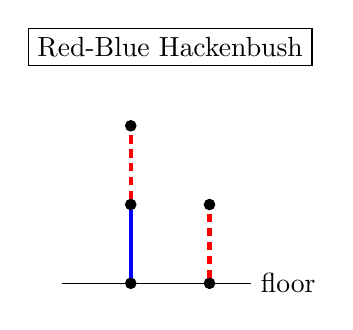
\begin{tikzpicture}
	\node[draw] (title) at (1.5, 3) {Red-Blue Hackenbush};
	\node (p1) at (0,0) {};
	\node (p2) at (3,0) {floor};
	\begin{scope} [every node/.style={scale=0.4, circle, draw, fill=black}]
	\node (p3) at (1,0) {};
	\node (p4) at (1,1) {};
	\node (p5) at (1,2) {};
	\node (p6) at (2,0) {};
	\node (p7) at (2,1) {};
	\draw (p1) -- (p2);
	\begin{scope} [ultra thick]
	\draw[blue] (p3) -- (p4);
	\draw[red, densely dashed] (p4) -- (p5);
	\draw[red, densely dashed] (p6) -- (p7);
	\end{scope}
	\end{scope}
	\end{tikzpicture}
\end{center}
\caption{The first instance of a combinatorial game}
\end{figure}

In Red-Blue Hackenbush, or RB-Hackenbush, a move is made by removing a single colored edge of the image and any other edges that become disconnected from the floor. The player called Left can only remove bLue and soLid, edges, and the other, called Right, RED and dashED edges. It is a common practice to assume that all games are played between Left and Right and that if necessary the same color scheme will be used, although, occasionally, new colors will be presented.

The RB-Hackenbush is a game by the routine definition of game, meaning it has a clear ruleset and potential to be fun. It is also a game by the definition above, which will be the new routine one used going forward. However, the instance of this game drawn above is also called a game. In the future, when analyzing a board state for example, the word position is used interchangeably with the word game. Deciding which meaning the word game has must be deduced from context.

The following image depicts the fundamental process for analyzing a game with the lenses of combinatorial game theory.

\begin{figure} [H]
\begin{tikzpicture}
[
	sibling distance=150pt,
	level distance=100pt,
	level 1/.style={sibling distance=6cm},
	level 2/.style={sibling distance=3cm},
	every node/.style = {
			shape=rectangle,
			rounded corners,
			draw,
			align=center,
			top color=white,
			bottom color=blue!20
		},
	every child/.style = {
		ultra thick
	}
]
\node[] (title) at (0, 3) {Game Tree};
\coordinate (p1) at (0.5,0);
\coordinate (p2) at (2.5,0) {};
\node {
	\begin{tikzpicture}
	[
		every node/.style = {
			scale=0.4,
			circle,
			draw,
			fill=black
		},
		ultra thick
	]
			\node (p3) at (1,0) {};
			\node (p4) at (1,1) {};
			\node (p5) at (1,2) {};
			\node (p6) at (2,0) {};
			\node (p7) at (2,1) {};
			\draw (p1) -- (p2);
			\draw[blue] (p3) -- (p4);
			\draw[red, densely dashed] (p4) -- (p5);
			\draw[red, densely dashed] (p6) -- (p7);
	\end{tikzpicture}
}
child [draw=blue] {
	node [thin, black] {
	\begin{tikzpicture}
	[	
		every node/.style = {
			scale=0.4,
			circle,
			draw,
			fill=black
		},
		ultra thick
	]
	\node (p6) at (2,0) {};
	\node (p7) at (2,1) {};
	\draw (p1) -- (p2);
	\draw[red, densely dashed] (p6) -- (p7);
	\end{tikzpicture}} 
	child [draw=red, dashed] {node [thin, solid, black] {} } }
	child [draw=red, dashed] {node [thin, solid, black] {
		\begin{tikzpicture}
		[	
		every node/.style = {
			scale=0.4,
			circle,
			draw,
			fill=black
		},
		ultra thick
		]
		\node (p3) at (1,0) {};
		\node (p4) at (1,1) {};
		\node (p5) at (1,2) {};
		\draw (p1) -- (p2);
		\draw[blue] (p3) -- (p4);
		\draw[red, densely dashed] (p4) -- (p5);
		\end{tikzpicture}
}
	child [draw=blue, solid] {node [thin, black] {} }
	child [draw=red, dashed] {node [thin, solid, black] {
			\begin{tikzpicture}
			[	
			every node/.style = {
				scale=0.4,
				circle,
				draw,
				fill=black
			},
			ultra thick
			]
			\node (p3) at (1,0) {};
			\node (p4) at (1,1) {};
			\draw (p1) -- (p2);
			\draw[blue] (p3) -- (p4);
			\end{tikzpicture}
	}
	child [draw=blue, solid] {node [thin, black] {} }
	}
}
child [draw=red, dashed] {node [thin, solid, black] {
		\begin{tikzpicture}
		[	
		every node/.style = {
			scale=0.4,
			circle,
			draw,
			fill=black
		},
		ultra thick
		]
		\node (p3) at (1,0) {};
		\node (p4) at (1,1) {};
		\node (p6) at (2,0) {};
		\node (p7) at (2,1) {};
		\draw (p1) -- (p2);
		\draw[blue] (p3) -- (p4);
		\draw[red, densely dashed] (p6) -- (p7);
		\end{tikzpicture}
} 
	child [draw=blue, solid] {node [thin, solid, black] {
			\begin{tikzpicture}
			[	
			every node/.style = {
				scale=0.4,
				circle,
				draw,
				fill=black
			},
			ultra thick
			]
			\node (p6) at (2,0) {};
			\node (p7) at (2,1) {};
			\draw (p1) -- (p2);
			\draw[red, densely dashed] (p6) -- (p7);
			\end{tikzpicture}
}
child [draw=red, dashed] {node [thin, solid, black] {} } }
	child [draw=red, dashed] {node [thin, solid, black] {
			\begin{tikzpicture}
			[	
			every node/.style = {
				scale=0.4,
				circle,
				draw,
				fill=black
			},
			ultra thick
			]
			\node (p3) at (1,0) {};
			\node (p4) at (1,1) {};
			\draw (p1) -- (p2);
			\draw[blue] (p3) -- (p4);
			\end{tikzpicture}
}
	child [draw=blue, solid] {node [thin, black] {} } }};
\end{tikzpicture}
\caption{Method used to build a game tree}
\end{figure}


The game tree is a term commonly used to refer to a graph containing all the possible outcomes of each move. The tree used may be slightly different as in each configuration both players' move are considered, regardless of who is the next to play. The image above is the game tree that arises from the game presented in \textit{Figure 2.1}.

In the tree above the styled edges, in the same pattern as before, between configurations tell which player made a move. As noted previously, the game tree contains all the information required to analyze games. Consider that analyzing a game is the same as calculating the number, or non-number, a game is equal to, like suggested in the introduction.

Again from the introduction, it is known that there is a most natural way to add two games together. This possibility comes from the fact that it is possible to easily merge together the game trees, as they are used in the figure. The addition of two games is equal to the merge of the two game trees. This merge is done by making the left and right options equal to the union of the left and right options of the summands.

Notice that in the case of the figure it is possible to consider that the whole game is actually the sum of two separate games. Each component is a graph connected to the floor, namely
\scalebox{0.5}{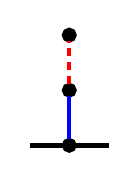
\begin{tikzpicture}
	[
	every node/.style = {
		scale=0.4,
		circle,
		draw,
		fill=black
	},
	ultra thick
	]
	\node (p1) at (1,0) {};
	\node (p2) at (1,0.7) {};
	\node (p3) at (1,1.4) {};
	\draw (0.5,0) -- (1.5,0);
	\draw[blue] (p1) -- (p2);
	\draw[red, densely dashed] (p2) -- (p3);
\end{tikzpicture}} and 
\scalebox{0.5}{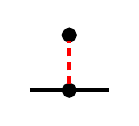
\begin{tikzpicture}
		[
		every node/.style = {
			scale=0.4,
			circle,
			draw,
			fill=black
		},
		ultra thick
		]
		\node (p1) at (1,0) {};
		\node (p2) at (1,0.7) {};
		\draw (0.5,0) -- (1.5,0);
		\draw[red, densely dashed] (p1) -- (p2);
\end{tikzpicture}}, because they are both disconnected.
Also, notice how the game tree is in fact the merge of the components' game trees.

To complete the analysis of the game above, the next step is to decide if it is a number or not. The definition of Surreal Numbers, the only class that contains all games that are numbers, has a recursive nature that can be completely separated from games. However, as they were created analyzing a position like the one above~\cite{CGT}, it makes sense to present it in the original terms, counting spare moves.

The model Conway, Berlekamp and Guy created to analyze games is based on finding the advantage a player has over the other. According to this model, the calculation of this advantage is given in terms of spare moves. When analyzing games it is important to expect that both players play perfectly, so the number of spare moves is calculated considering that both parts take optimal decisions. Since a player loses if he or she cannot move, counting spare moves is counting how many sequential moves a player can make before reaching equity in the position.

Equity is found in zero positions. Zero positions are those in which the first player to move loses. The idea to call such positions zero made sense for Conway, and, therefore, in his new set of numbers, if a game \Gm{} is in a zero position, \Gm{=0}. If Left can win regardless of who starts, the number is called positive, and, if Right wins, negative. In more special positions, a hint on the topic of this text, in which the first to play can win, positions are called fuzzy.

\begin{figure} [H]
	\begin{center}
		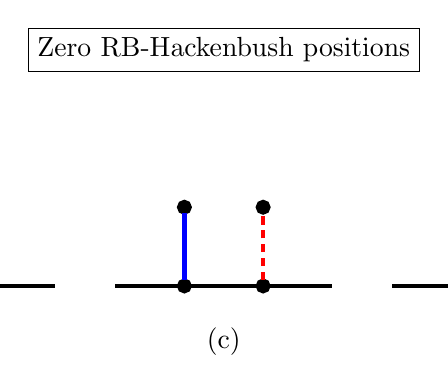
\begin{tikzpicture}
			\node[draw] (title) at (1.5, 3) {Zero RB-Hackenbush positions};
			\node (p1) at (0,0) {};
			\node (p2) at (3,0) {};
			\begin{scope} [ultra thick, every node/.style={scale=0.4, circle, draw, fill=black}]
				\node (p3) at (1,0) {};
				\node (p4) at (1,1) {};
				\node (p6) at (2,0) {};
				\node (p7) at (2,1) {};
				\draw (p1) -- (p2);
				\draw[blue] (p3) -- (p4);
				\draw[red, densely dashed] (p6) -- (p7);
			\end{scope}
			\coordinate[thick, label=(c)] () at (1.5, -1);
			\hspace{-200pt}{ \begin{scope} [ultra thick, every node/.style={scale=0.4, circle, draw, fill=black}]
				\draw (p1) -- (p2);
			\end{scope}}
			\coordinate[thick, label=(a)] () at (1.5, -1);
			\hspace{100pt}{ \begin{scope} [ultra thick, every node/.style={scale=0.4, circle, draw, fill=black}]
				\node (p3) at (1,0) {};
				\node (p4) at (1,1) {};
				\node (p5) at (1,2) {};
				\node (p6) at (1.5,0) {};
				\node (p7) at (1.5,1) {};
				\node (p8) at (2, 0) {};
				\node (p9) at (2, 1) {};
				\draw (p1) -- (p2);
				\draw[blue] (p3) -- (p4);
				\draw[blue] (p4) -- (p5);
				\draw[red, densely dashed] (p6) -- (p7);
				\draw[red, densely dashed] (p8) -- (p9);
			\end{scope}}
			\coordinate[thick, label=(b)] () at (1.5, -1);
			\hspace{200pt}{ \begin{scope} [ultra thick, every node/.style={scale=0.4, circle, draw, fill=black}]
				\node (p3) at (1,0) {};
				\node (p4) at (1,1) {};
				\node (p5) at (1,2) {};
				\node (p6) at (2,0) {};
				\node (p7) at (2,1) {};
				\node (p8) at (2,2) {};
				\draw (p1) -- (p2);
				\draw[blue] (p3) -- (p4);
				\draw[red, densely dashed] (p4) -- (p5);
				\draw[red, densely dashed] (p6) -- (p7);
				\draw[blue] (p7) -- (p8);
			\end{scope}}
			\coordinate[thick, label=(d)] () at (1.5, -1);
			\hspace{100pt}{ \begin{scope} [ultra thick, every node/.style={scale=0.4, circle, draw, fill=black}]
				\node (p3) at (1,0) {};
				\node (p4) at (1,1) {};
				\node (p6) at (2,0) {};
				\node (p7) at (2,1) {};
				\node (p8) at (1.5,2) {};
				\draw (p1) -- (p2);
				\draw[blue] (p3) -- (p4);
				\draw[red, densely dashed] (p4) -- (p8);
				\draw[red, densely dashed] (p6) -- (p7);
				\draw[blue] (p7) -- (p8);
			\end{scope}}
			\coordinate[thick, label=(e)] () at (1.5, -1);
		\end{tikzpicture}
	\end{center}
	\caption{Several instances of 0 positions in RB-Hackenbush}
\end{figure}

Although all games have the same value, the games are not the same because their game tree is different. Moving forward, there is a new way to represent a game that derives directly from its game tree. The game is composed of two sets of games and $\mid$ is used as delimiter between the sets. The game (a) is one where neither player has available moves and, because of that, the game $(a) = 0 = \gam{}{}$. On the other had, $(c) = 0 = \gam{\gam{}{\gam{}{}}}{\gam{\gam{}{}}{}}$, that simplifies to \gam{\gam{}{0}}{\gam{0}{}}. The games that form each of the left and right sets are the configurations reached after Left and Right make a move, in a recursive definition.

The notation is exactly the same for numbers, but they should not be confused. For a game  \Gm{= \gam{X}{Y}} to be a number, it must be true that $X < Y$, meaning:
\hspace{-0.5cm}
$$x < y, \mbox{for all $x$ in $X$ and $y$ in $Y$}$$

The process of finding the number a game is thoroughly discussed to is the theme of the next section. With that said, some new numbers already showed up in the figure above. The number \gam{0}{}, for example. What would be a pleasant real number for it? 1, because in this game, left has exactly one move to spare.

For the next few concepts a new game must be presented as RB-Hackenbush is incapable of generating fuzzy positions, the reason why all such games are numbers will be provided in the next section. It is worth for the reader trying to create any instance of fuzzy position in this game to accept it for th meantime.

\begin{figure} [!ht]
	\begin{center}
		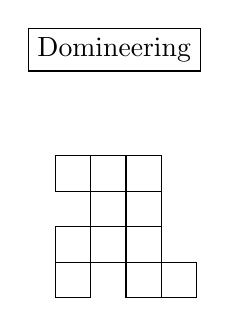
\begin{tikzpicture}[scale=1.5]
		\node[draw] (title) at (0.5, 1.8) {Domineering};
		\draw[] (0,-0.3) rectangle ++(0.3,0.3);
		\draw[] (0,0) rectangle ++(0.3,0.3);
		\draw[] (0,0.6) rectangle ++(0.3,0.3);
		\draw[] (0.3,0) rectangle ++(0.3,0.3);
		\draw[] (0.3,0.3) rectangle ++(0.3,0.3);
		\draw[] (0.3,0.6) rectangle ++(0.3,0.3);
		\draw[] (0.6,-0.3) rectangle ++(0.3,0.3);
		\draw[] (0.6,0) rectangle ++(0.3,0.3);
		\draw[] (0.6,0.3) rectangle ++(0.3,0.3);
		\draw[] (0.6,0.6) rectangle ++(0.3,0.3);
		\draw[] (0.9,-0.3) rectangle ++(0.3,0.3);
		\end{tikzpicture}
	\end{center}
	\caption{The first game that is hot}
\end{figure}

Domineering is played by placing, or marking, a $2\times1$ rectangle on the board, or drawing. Left plays in the vertical and right in the horizontal. The reader is invited to play the position above a few times, and realize that the player starting it is always able to win. In fact, with perfect play, both players can win with a move to spare. The quest for calculating the advantage a player has, so far, can be been summarized by the question: ``Who is ahead, by how much?". However, in positions such as the one above, a new question is more important: ``How big is the next move"~\cite{6}.

This second question is answered in temperature theory. Temperature theory must follow a detailed explanation and clear understanding of numbers and games, and, therefore, a good explanation will only take place in section 4. However, as this is the main tool used to develop the topic of this text, the intuition or idea follows in the remaining of this chapter. The examples will use the game of chess because it is a widely known combinatorial game and serves well the purpose. Chess, however, is not a short game, as, although it is a finite game, it is not loopfree.

Temperature measures the activity of a position. Activity should be understood as the importance of the next move. To make an analogy, in chess, for example, closed positions would be colder than endgame positions. In the position below, being the next player to move is not that important. Both players would start improving the position of the pieces until one finds a break-through. Being a move behind means less piece development but the game will progress slowly, reducing the impact of that.

\begin{center}
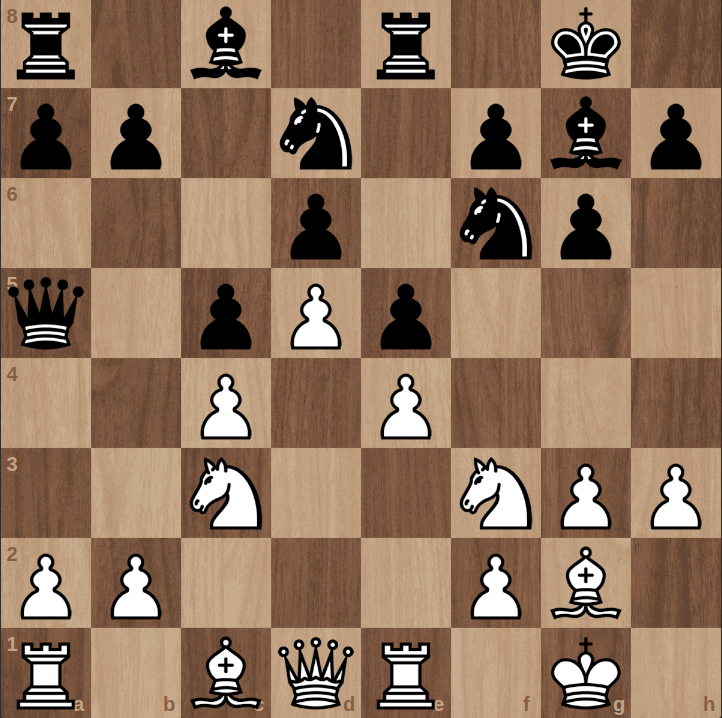
\includegraphics[scale=0.15]{images/chess_cold} 
\end{center}

In hot positions, opposed to cold position, the next moves are paramount for both players. In the board below, the player who moves first has a clear path to victory. In case chess rules are not known, in the position below White can move the pawn one square forward and that results in a promotion. White promotes to a queen and regardless of Black's move, White can soon capture the pawn, resulting in a straight-forward win for White. The same can be said for Black if he/she starts.

\begin{center}
	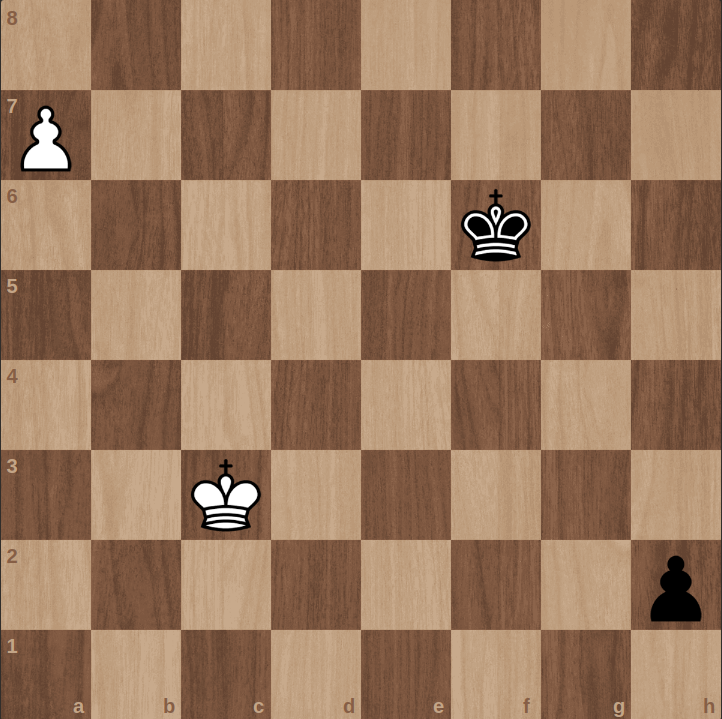
\includegraphics[scale=0.15]{images/chess_hot} 
\end{center}

It is correct to imagine that when writing hot game \Gm{} in the notation \Gm{= \gam{X}{Y}}, then, $X \nleq Y$, which implies that there are left and right options \Gm{^L} and \Gm{^R} such that $\Gm{^L} \ge \Gm{^R}$, making it obvious that \Gm{} is not a number. On the closed position, the game might be cooler, but it will definitely heat up after a few moves. The endgame position above however, is cooling down completely, becoming a number, after the next move. Because both Left and Right options are numbers, it receives the special name of switch.

Switches are the most basic non-numbers. A switch is a non-numbers \Gm{} that both left's and right's best moves are numbers, but $G^L \ge G^R$. It is extremely easy to find the temperature and bias of such games. The process is shown here and will be used in again in the future.

\begin{figure} [!ht]
	\begin{center}
		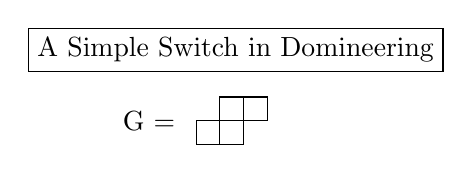
\begin{tikzpicture}
			\node[draw] (title) at (0.5, 0.9) {A Simple Switch in Domineering};
			\node (title) at (-0.6, 0) {G = };
			\draw[] (0.3,-0.3) rectangle ++(0.3,0.3);
			\draw[] (0.3, 0) rectangle ++(0.3,0.3);
			\draw[] (0.6, 0) rectangle ++(0.3,0.3);
			\draw[] (0,-0.3) rectangle ++(0.3,0.3);
		\end{tikzpicture}
	\end{center}
	\caption{The first game that is a switch}
\end{figure}

In this game left has a move that leads to a zero position and right has two moves that lead to the same game with value -1. Therefore, \Gm{= \gam{0}{{-}1}}. The bias is the average of $G^L$ and $G^R$, which is equal to $-0.5$ in this case. The temperature is how much the left and right values differ from the bias, which is $0.5$ in this example. A better way of writing this switch is $G = -0.5 \pm 0.5$. In general, a switch $H = \gam{x}{y}$ can be written as $H = (x+y)/2 \pm (x-y)/2$. 

Calculating these values for general non-numbers is more demanding. The temperature of a general hot game is calculated based on its subpositions temperatures and the process of cooling them. This process is visualized through a temperature graphic called thermograph.

Although building thermographs is simple and cooling sounds harder than it is, these concepts are saved for later. They do not fit introductory pages because better understanding of numbers and arithmetic is required. With that said, there is one important detail that might have gone unnoticed until this point.

It was said that numbers can be added together, because the game trees are able to be merged together. However, merging game trees is more general than adding numbers, so the reality is that not just the numbers, but all games can be summed using the same procedure. If \Gm{} and \Hm$\,$ are games, \Gm{ + \Hm} is a game and it is defined by $\Gm{ + \Hm = \gam{G^{L_I}+H, G+H^{L_I}}{G^{R_I}+H, G+H^{R_I}}}$, where \Gm{^{L_I}} is used to denote all possible Left's moves in \Gm{} and the remaining is defined in a similar fashion.

Notice that game addition is used to define addition itself, but that is a consequence of the recursive nature of games. After a finite number of steps, all of $\Gm{^{L_I}}, \Hm^{L_I}, \Gm{^{R_I}}, \Hm^{R_I}$ become empty, finishing the recursive structure. Therefore it is possible to add together numbers and non-numbers, but the properties of this operation are only described and used in the next chapters.







